\documentclass[a4paper,11pt]{article}

\usepackage{lipsum}
\usepackage{titling}
\usepackage{exptech}       

\usepackage{graphicx}

\usepackage{pgfplots}
\pgfplotsset{compat=1.13}





\title{ \textbf{Apprentissage incrémental de règles de décision} }
\markright{\thetitle} 
\author{Bassirou \textsc{Seye}, Clément \textsc{Fournier}, \\
        Léandre \textsc{Le Polles -{}- Potin}, Pierre \textsc{Testart} \\
        \\
        Encadreur : Laurence \textsc{Rozé}}

\date{}                    

\def\antd#1{\texttt{#1}}

\begin{document}          

    \maketitle                 
    \thispagestyle{empty}      

    \begin{abstract}

        Notre projet avait pour but d'implémenter un algorithme d'apprentissage incrémental de règles de décision appelé VFDR, décrit dans \cite{Gama-VFDR}. Pour ce faire, nous nous sommes servis de l’API de Weka, une plate-forme d'apprentissage artificiel qui propose de nombreux algorithmes d'apprentissage et de classification. 
        
    \end{abstract} 

    \section{Introduction}

    \subsection{Notions d'apprentissage artificiel}

        Pour introduire les notions principales nécessaires à la compréhension du travail accompli, nous allons prendre un exemple qui nous servira de fil directeur : l’exemple classique de la différenciation entre les oies et les cygnes. La question posée est la suivante : «~Comment un programme peut-il apprendre à différencier ces deux oiseaux~?~»

        \subsubsection{Règles de décisions}

            La classification est une tâche qui consiste à attribuer une étiquette (que l'on appelle \emph{classe}) à un individu qui n'en possède pas. Notre exemple des oiseaux est un exemple de classification: à partir de données sur un oiseau, on doit déterminer s'il s'agit d'une oie ou d'un cygne. Dans les algorithmes qui utilisent des règles, on base la décision d'attribuer une étiquette particulière à l'individu sur la validation de certaines \emph{règles}, c'est-à-dire la validation simultanée d'une ou plusieurs conditions sur les données qui décrivent l'individu à classifier.

            Les données qui décrivent chaque individu sont les valeurs associées à des caractéristiques mesurables de l'individu, que l'on appelle des \emph{attributs}. Par exemple, pour nos oiseaux, la taille en centimètres est un attribut numérique (il prend ses valeurs dans un ensemble ordonné et potentiellement infini) et la couleur du plumage est un attribut nominal (il prend ses valeurs dans un ensemble fini et non-ordonné, ici \["clair", "moyen", "sombre"\]). Les attributs nominaux et numériques sont les deux types de données que notre algorithme supporte.

            Les règles qui nous permettent de prendre une décision de classification se présentent sous la forme de conjonctions de conditions sur les attributs de l'individu à classifier. On appelle ces conditions des \emph{littéraux} (ou \emph{antécédents}). Pour des attributs numériques, on compare la valeur avec des valeurs seuils. Ainsi, un antécédent numérique pourrait être \antd{taille > 50cm}. Les valeurs des attributs nominaux n'étant pas ordonnées, les antécédents nominaux sont de la forme \antd{plumage = clair}.

            Une règle permettant de classifier les oiseaux peut se présenter de la façon suivante : « Si \antd{plumage = "clair"} et \antd{taille > 140}, alors \antd{classe = "cygne"}. » Lorsque l'on tente de classifier un individu qui n'a pas d'étiquette, on lui attribue donc la classe "cygne" s'il vérifie les conditions de la règle. Si c'est le cas, on dit qu'il est \emph{couvert} par la règle.

            Exprimer une règle sous la forme «~Si <suite de littéraux> alors <classe>~» est en fait une simplification du fonctionnement des règles de décision utilisées par VFDR. En réalité, nos règles stockent, pour chaque classe, des statistiques sur les individus couverts appartenant à cette classe. Lorsqu’un individu non-étiqueté est couvert par une règle, on ne peut donc pas décider immédiatement de sa classe, on utilise pour cela une stratégie de classification (plus d'explications en section \ref{ssec:nondecisional}).


        \subsubsection{Apprentissage}\label{ssec:apprentissage}

           Le but d'un algorithme d'apprentissage est de constituer un ensemble de règles qui décrivent au mieux les individus déjà observés pour avoir une estimation de la classe d'un nouvel individu à classifier. Pour entraîner un tel algorithme, c'est-à-dire pour qu'il construise un modèle pertinent, on lui fournit un \emph{échantillon d'apprentissage} constitué d'individus déjà étiquetés. Pour notre exemple des cygnes et des oies, on peut représenter un échantillon d'apprentissage sur un diagramme comme celui présenté en figure \ref{fig:example}. À partir de ces données, il se dégage que la plupart des oiseaux au plumage clair sont des cygnes, et tous les oiseaux au plumage sombre sont des oies. De plus, les cygnes sont plus grands que les oies en général. En conséquence, un ensemble de règles à peu près pertinent pourrait être:
            \begin{itemize}
                \item Si \antd{plumage = "clair"} et \antd{taille > 140}, alors \antd{classe = "cygne"};
                \item Si \antd{plumage = "moyen"} et \antd{taille > 170}, alors \antd{classe = "cygne"};
                \item Si \antd{plumage = "sombre"}, alors \antd{classe = "oie"};
                \item Sinon \antd{classe = "oie"}.
            \end{itemize}
            \begin{figure}\centering
                \begin{tikzpicture}
                    \begin{axis}[%
                        scale=.8,
                        scale only axis,
                        xlabel={\texttt{Taille (cm)}},
                        ytick={0,1,2},
                        yticklabels={clair,moyen,sombre},
                        ylabel={\texttt{Plumage}},
                        cycle list name=black white,
                    %   xmajorticks=false,
                        ymajorgrids,]
                  %     legend style={at={(0.97,0.03)},anchor=south east,nodes=right}]
                       \addplot table [scatter, only marks,header=false,col sep=comma] {src/geese.csv};

                        \addlegendentry{Oies};

                        \addplot table [scatter, only marks, header=false,col sep=comma] {src/swans.csv};

                        \addlegendentry{Cygnes};
                    \end{axis}
                \end{tikzpicture}
                \caption{Exemple d'échantillon d'apprentissage à deux attributs : \texttt{Plumage} est nominal, \texttt{Taille} est numérique. Chaque point représente un individu, sa position dénote la valeur de ses attributs.}
                \label{fig:example}
            \end{figure}



        \subsubsection{Incrémentalité}

            Les algorithmes d’apprentissage incrémentaux sont capables de mettre à jour les règles de décision à chaque individu catégorisé fournit, tout en laissant la possibilité à tout moment d’utiliser lesdites règles de décision pour classifier un individu dont on ne connaît pas encore la classe.

            Ces algorithmes sont conçus pour optimiser leur utilisation d'espace mémoire et le temps qu'ils mettent à classifier une instance, et sont donc adaptés à l'apprentissage sur des flux de données importants et continus.

    \subsection{Weka}

        Weka (Waikato Environment for Knowledge Analysis) est une plate-forme d'apprentissage artificiel, programmée en Java, permettant de réaliser de nombreuses tâches d’apprentissage et de classification. Elle rend accessible les différentes techniques de Data Mining et de Machine Learning et  permet d’appliquer rapidement ces techniques sur des problèmes concrets. Elle propose aussi une API très complète pour l'implémentation de nouveaux algorithmes.

    \section{Présentation de VFDR}

        L’algorithme VFDR, sigle de «~Very Fast Decision Rules~», est l’algorithme d’apprentissage incrémental de règles qui nous intéressera ici. Nous allons dans ce chapitre décrire le fonctionnement de cet algorithme.

        \subsection{Principe}

            L’algorithme commence avec un ensemble vide de règles et une règle par défaut. Cette règle, ne comprenant aucun littéral, couvre tous les individus qui ne sont couverts par aucune autre règle. On peut l'exprimer par «~Sinon...~» comme dans l'exemple d’ensemble de règles de la section \ref{ssec:apprentissage}. À chaque règle est associée une structure de données permettant de calculer les statistiques nécessaires au traitement de ladite règle.

            Lorsque l’algorithme reçoit un individu étiqueté, il tente de le faire correspondre à chaque règle de l’ensemble de règles ou à la règle par défaut. Si la règle qui le couvre contient suffisamment d’individus, elle est étendue pour améliorer sa précision. L’extension d’une règle consiste à lui rajouter un littéral. Lorsque c’est la règle vide qui devrait être étendue, une nouvelle règle est créée à la place. Ainsi, l’algorithme construit l’ensemble de règles qui servira à classifier les individus non étiquetés.

        \subsection{Statistiques suffisantes}\label{ssec:stats}

            Pour ne pas saturer la mémoire, l’algorithme ne mémorise pas l’ensemble des individus traités, mais utilise une structure de données contenant des statistiques sur les individus couverts par la règle.

            Cette structure de données, que l’on appelle les \emph{statistiques suffisantes}, est constituée de :
            \begin{itemize}
                \item Un entier correspondant au nombre d’individus couverts par la règle;
                \item Un vecteur d’entiers stockant le nombre d’occurrences de chaque classe parmi les individus couverts (distribution de classes);
                \item Une matrice représentant le nombre d'occurrences de chaque valeur des attributs nominaux pour chaque classe;
                \item Un estimateur gaussien par classe, permettant de calculer pour chaque attribut numérique la probabilité de rencontrer une valeur supérieur à une valeur déjà rencontrée.
            \end{itemize}

            Prenons l’exemple des oies et des cygnes. Nous lançons l'algorithme sur les sept individus suivants :

            \begin{table}[h]\centering
                \begin{tabular}{|ccc|}\hline
                    Classe&Plumage&Taille (cm)\\ \hline
                	Oie & sombre & 76 \\
                	Oie & moyen & 82 \\
                	Oie & moyen & 78 \\
                	Cygne & moyen & 112 \\
                	Cygne & clair & 90 \\
                	Cygne & moyen & 98 \\
                	Cygne & clair & 86 \\ \hline
                \end{tabular}
            \end{table}

            Ces individus sont couverts uniquement par la règle vide, car trop peu d'individus ont été rencontrés pour créer de nouvelles règles. La structure de données de la règle vide contient donc les valeurs suivantes :
            \begin{itemize}
                \item Nombre d’individus couverts : 7
                \item Distribution de classe : \texttt{["oie": 3, "cygne": 4]}
                \item Matrice de valeurs nominales : %\\
                    
                    \begin{table}[h]\centering
                        \begin{tabular}{|l|cc|}\hline
                            & \antd{classe = oie} & \antd{classe = cygne}\\ \hline
                        \antd{plumage = sombre}  & 1 & 0 \\
                        \antd{plumage = moyen}   & 2 & 2 \\
                        \antd{plumage = clair}   & 0 & 2 \\\hline
                        \end{tabular}
                    \end{table}%\vspace{4mm}
                
                \item Les estimateurs gaussiens de chaque classe sont ajustés pour correspondre aux valeurs de taille rencontrées.
            \end{itemize}

            Ainsi, à chaque ajout d’un individu couvert par la règle, il suffit de mettre à jour les statistiques pour garder en mémoire les informations importantes. L’ensemble de règles construit par VFDR peut être \emph{ordonné} ou \emph{non-ordonné}. Dans le premier cas, seule la première règle qui couvre l’individu est mise à jour. Dans le second cas, toutes les règles couvrant l’individu sont mises à jour et éventuellement étendues. Cependant, dans les deux cas de figure, la règle par défaut n’est mise à jour que si \emph{aucune} autre règle ne couvre l’individu.

            Quand une règle atteint le nombre seuil d’individus défini précédemment, l’algorithme procède à l'expansion de cette règle.

        \subsection{Expansion d'une règle}

            Lors de l’expansion d’une règle, on cherche à lui ajouter un littéral de sorte que la distribution de classes de la règle étendue soit la plus pure possible, c’est-à-dire qu’une classe en particulier y soit plus représentée. Ceci permet de prendre de meilleures décisions, puisqu’il y aura une plus forte certitude qu’un individu couvert par cette règle appartienne à la classe majoritairement représentée. À cet effet, on utilise une mesure de la pureté d’une distribution de classe que l’on appelle \emph{entropie}. Une distribution de classe parfaitement pure aura une entropie nulle, on cherche donc à la minimiser.
            
            Pour décider si l'on étend une règle ou pas, on compare la valeur de l'entropie à une limite qu'on appelle la \emph{borne de Hoeffding}. Si la valeur est supérieure à la borne, cela signifie que la règle n'est plus pertinente. On procède alors à l'expansion de la règle, dans l'espoir qu'une expansion la fasse gagner en pureté. Dans le cas contraire, on reporte juste l'expansion à plus tard.

            Pour étendre une règle, l’algorithme cherche le littéral qui minimise l’entropie de la distribution de classes \emph{a priori} de la règle étendue. Cela implique de trouver à la fois l’attribut et la valeur sur lequel on va le tester. Parmi tous les attributs qui n’appartiennent à aucun littéral de la règle, on cherche alors la valeur de test qui produira l’entropie la plus faible dans la distribution, estimée grâce aux statistiques que l’on possède sur les attributs (stockées dans les statistiques suffisantes).

            Une fois le meilleur littéral construit, on vérifie que le gain de pureté obtenu par l'expansion de la règle est supérieur à la borne de Hoeffding. Si oui, on ajoute le nouveau littéral à la règle et on réinitialise ses statistiques. Les nouveaux individus couverts par la classe serviront à repeupler ces statistiques jusqu'à la prochaine extension de la règle.

        
        \subsection{Stratégies de classification}\label{ssec:nondecisional}
        
            On sait que chaque règle stocke la distribution de classes des individus qu'elle couvre. La classification d'un individu n'est donc pas automatique lorsqu'une règle le couvre, mais obéit à une \emph{stratégie de classification} que l'on peut paramétrer.

            La stratégie de classification la plus simple consiste à classer l’individu non-étiqueté dans la classe la plus représentée par la règle le couvrant, quelles que soient les valeurs de ses attributs. Mais cette stratégie ignore un bon nombre d’informations qui sont mises à disposition par l’algorithme. Une autre stratégie pourrait être de maximiser la probabilité de bon classement en utilisant l’ensemble des attributs de l’individu, par la méthode dite du «~bayésien naïf~».\cite{Gama-VFDR}
            
            Reprenons l’exemple de règle par défaut de la section \ref{ssec:stats}, dans le cas où un individu non étiqueté de couleur Sombre et mesurant 76 centimètres était traité par l’algorithme. Si la première stratégie de classification était utilisée, l’individu serait étiqueté comme étant de la classe «~oie~» car il s'agit de la classe majoritairement couverte par la règle. Cependant, en utilisant la stratégie du bayésien naïf, qui s'intéresse aux valeurs de ses attributs, on remarque qu’il est plus probable que l’individu soit en réalité de la classe «~cygne~». 

            Notre implémentation est paramétrable et laisse le choix à l'utilisateur d'utiliser le bayésien naïf ou non.

            Une seconde nuance que nous faisons dans la prise de décision dépend de la nature ordonnée ou non de l'ensemble de règles. Dans un ensemble de règle ordonné, seule la première règle couvrant l’individu décide de sa classification (stratégie \texttt{First Hit}), alors que pour un ensemble de règle non-ordonné, toutes les règles couvrant l’individu procèdent à un vote pondéré pour classifier l’individu (stratégie \texttt{Weighted Max}).






    \section{Travail réalisé}

    \subsection{Organisation} 

        Notre objectif pour ce second semestre d’étude pratique était d’implémenter l’algorithme. Nous avons décidé de travailler chacun de notre côté dans un premier temps, car nous ne connaissions pas suffisamment le fonctionnement de Weka et le travail semblait difficilement sécable. Cette approche nous a effectivement permis de nous familiariser individuellement avec la bibliothèque Weka et nous avons chacun travaillé sur un début d’implémentation de VFDR.

        Nous nous sommes ensuite réunis pour comparer nos avancées respectives et nos choix d’implémentation. Nous avons décidé de conserver les choix faits par Clément, pour des raisons de conception. C’est donc la base que nous avons utilisée pour terminer le travail du semestre.

    \begin{figure}
        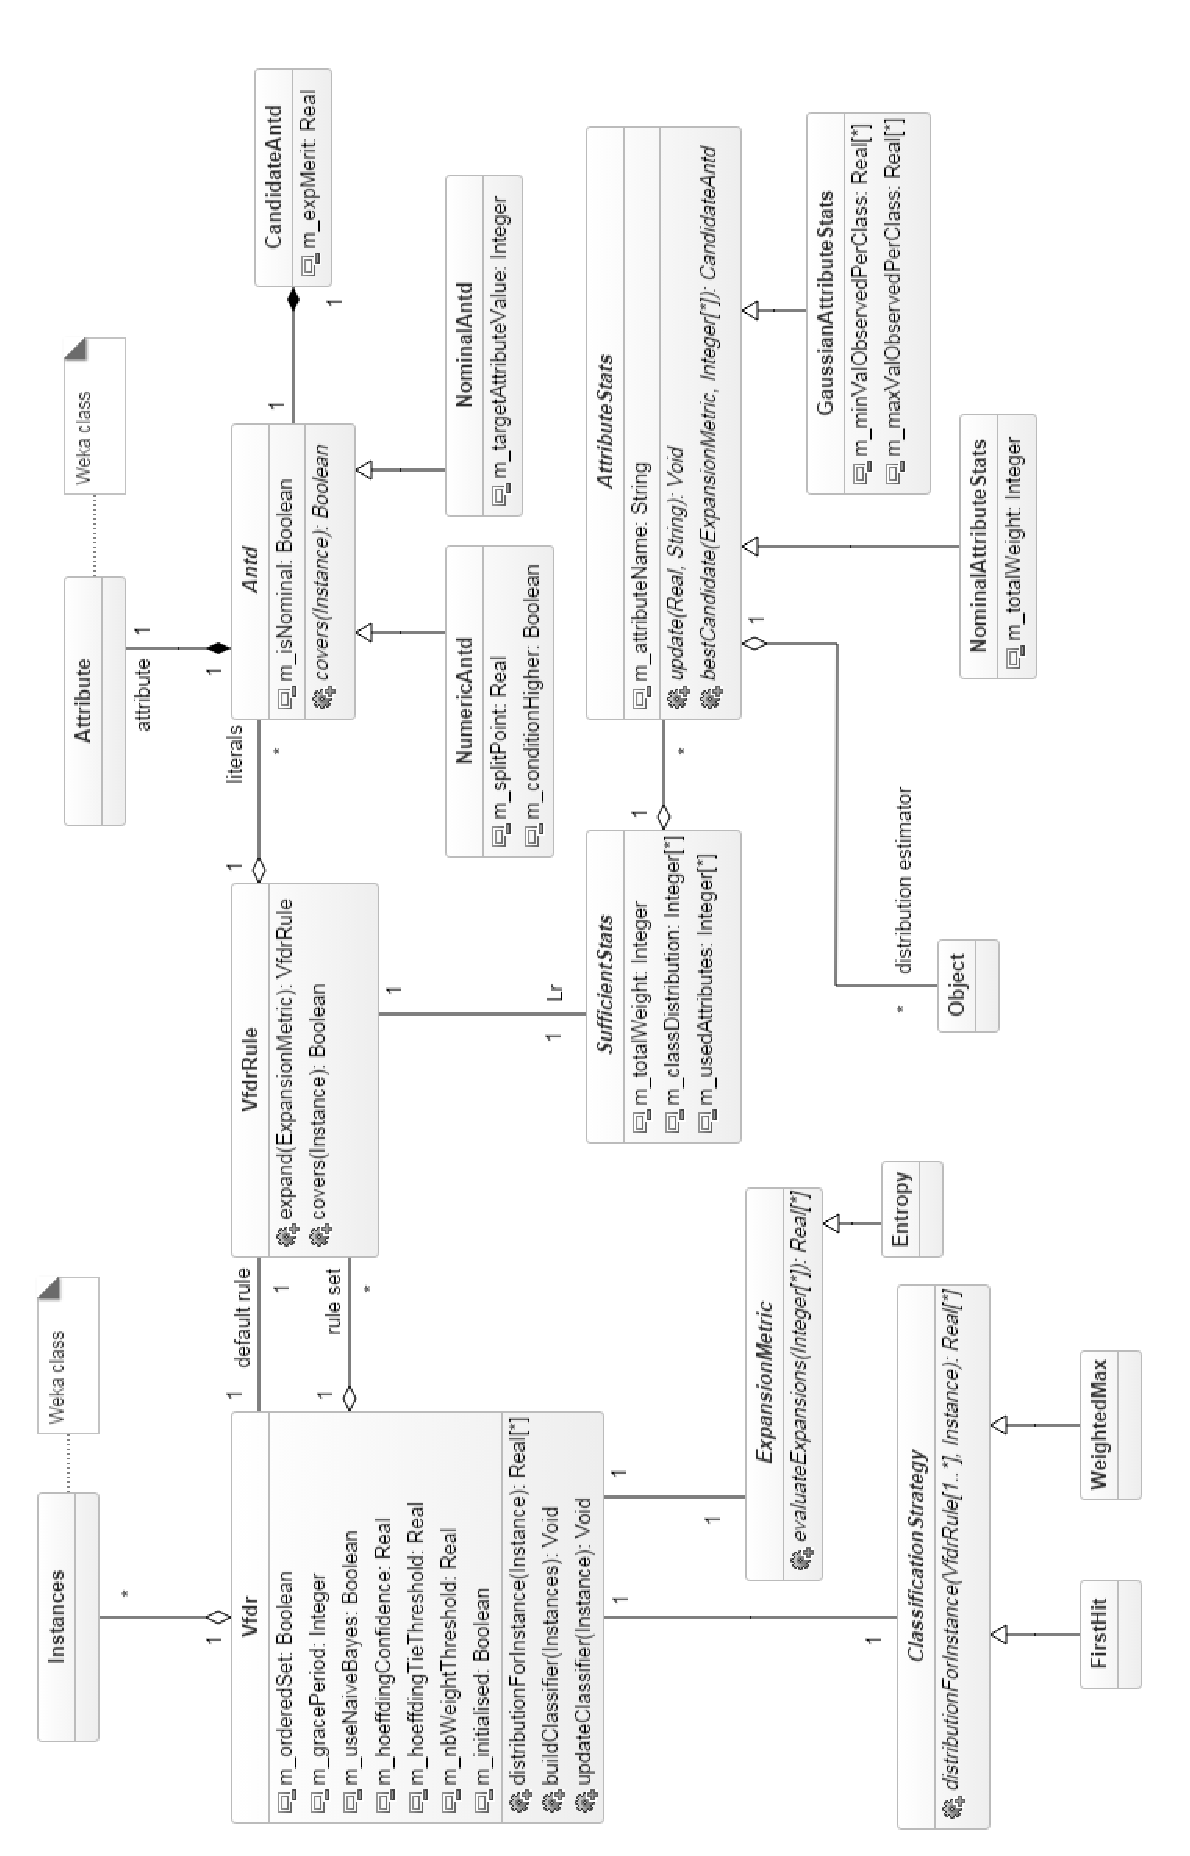
\includegraphics[width=\textwidth]{src/image2}
        \caption{Diagramme de classes de notre implémentation}
        \label{fig:dclass}
    \end{figure}


    \subsection{Description de l'implémentation}

        Le diagramme de classes en figure \ref{fig:dclass} présente l'architecture de notre implémentation.

        \paragraph{Paramétrage} La classe principale de notre programme, nommée \texttt{Vfdr}, implémente plusieurs interfaces de Weka, notamment \texttt{UpdateableClassifier}, qui permet de mettre en avant l’aspect incrémental de l’algorithme. Ces interfaces permettent d'intégrer le programme au GUI de Weka. \texttt{Vfdr} possède des attributs servant d’options de configuration, ainsi qu’une liste de \texttt{VfdrRule}, représentant l’ensemble des règles et une \texttt{VfdrRule} à part qui est la règle par défaut.

        \paragraph{Règles}Chaque objet \texttt{VfdrRule} possède lui-même une liste d’\texttt{Antd}, une classe abstraite servant à représenter les antécédents possibles pour les règles (spécialisée en \texttt{NumericAntd} pour les conditions sur les attributs numériques et \texttt{NominalAntd} pour les conditions sur les attributs nominaux). \texttt{VfdrRule} possède aussi une référence vers un objet \texttt{SufficientStats}, qui stocke les statistiques associées à la règle. 


        \paragraph{Statistiques suffisantes} 
            Dans l’implémentation, nous avons choisi d’identifier les classes des exemples par des Strings (le nom de la classe). Par conséquent, dans \texttt{SufficientStats}, le nombre d’exemples couverts par classe est stocké dans une \texttt{Map<String, Integer>}. Pour ce qui est des attributs, ils peuvent être représentés par des entiers (leur indice). On utilise par exemple une \texttt{List<Integer>} pour stocker les attributs déjà utilisés dans \texttt{SufficientStats}. Cependant, les attributs sont parfois identifiés par leur nom, comme les classes : les statistiques par attributs sont stockés dans une \texttt{Map<String, \texttt{AttributeStats}>}, où \texttt{AttributeStats} est une classe abstraite qui a des spécialisations différentes selon le type d’attribut.
            
            Pour gérer les statistiques des attributs numériques, certaines descriptions de l'algorithme VFDR indiquent d’utiliser un arbre binaire qui stocke pour chaque attribut la chance de rencontrer une valeur supérieure à chaque valeur déjà rencontrée. Pour simplifier l’implémentation, nous avons plutôt utilisé une densité de probabilité pour représenter les valeurs rencontrées : c’est la classe \texttt{GaussianAttributeStats}, qui hérite de \texttt{AttributeStats}. Les calculs sont faits dans la classe interne \texttt{GaussianEstimator}, qui hérite de la classe Weka \texttt{UnivariateNormalEstimator}. Ce choix a aussi l’avantage de limiter la complexité en temps et en espace.
        
        \paragraph{Expansion d'une règle} Pour l’expansion d’une règle, une liste de \texttt{CandidateAntd} (antécédents candidats) est créée. Le score de chaque candidat est évalué à l’aide d’un objet \texttt{ExpansionMetric}. Notons qu’\texttt{ExpansionMetric} est une classe abstraite, mais qu’elle n’a qu’une seule spécialisation possible : \texttt{Entropy}, qui utilise des calculs d’entropie pour évaluer la qualité d’une séparation. La mise en place d’une classe abstraite permet de laisser la possibilité d’améliorer l’implémentation, en ajoutant d'autres méthodes d’évaluation de séparation, tout en limitant les modifications à apporter au code existant.
        
        \paragraph{Prédiction} Lorsque l’on demande au \texttt{Vfdr} de classifier un exemple via la méthode \texttt{distributionForInstance}, sa stratégie de classification (représentée par la classe abstraite \texttt{ClassificationStrategy}) entre en jeu. Pour les ensembles ordonnés de règles, la stratégie est de type \texttt{FirstHit}, on renvoie la classe donnée par la première règle qui couvre l’exemple. Pour les ensembles non ordonnés, la stratégie est de type \texttt{WeightedMax}, on choisit alors la classe à partir de la règle qui couvre l’exemple et a le poids le plus élevé (le plus grand nombre total d’exemples couverts).

    \subsection{Limites de cette implémentation}

        Le temps de traitement d'un individu est suffisamment bas pour qu'il ne constitue pas un problème. Cependant la routine d'expansion de règle est très coûteuse et constitue le principal goulot d'étranglement pour le temps d'exécution du programme. Pour cette raison, nous avons défini une borne inférieure au nombre d'exemples que l'algorithme doit voir passer avant de tenter l'expansion. Cette limite est configurable et doit être adaptée au nombre d'exemples de l'échantillon d'apprentissage.

        L’algorithme ne peut pas gérer de changement de la fonction cible (ce que l'on appelle la \emph{dérive de concept}). Il existe une variante de l'algorithme qui peut s'y adapter, mais son implémentation était hors du champ de cette étude pratique.

    \section{Conclusion} 
        
       Au terme de ce projet d'études pratiques, nous disposons d'une implémentation de l'algorithme VFDR fonctionnelle. Après un bref échange avec Mark Hall, l'administrateur du projet libre Weka, notre implémentation a été intégrée dans le dépôt de modules officiel de Weka. Notre travail est donc libre d'accès à tout utilisateur du logiciel. 

	   Ce projet nous a permis de manipuler concrètement des notions de classification et d'apprentissage, nous en apprenant beaucoup sur ces sujets. Ayant dû lire de nombreux articles scientifiques afin de finaliser notre implémentation, nous avons également découvert le monde de la recherche. Enfin, malgré les limites de notre implémentation, ce projet nous a ouvert au monde de l'open-source, nous permettant à tous de contribuer pour la première fois à un logiciel libre de droits. Nous avons donc beaucoup appris de ce projet, tant sur le plan théorique que concret.

    \nocite{*}
    \bibliography{biblio}


\end{document}
